\section{Estudios de caso representativos}

Para ilustrar cómo los métodos y factores antes descritos se aplican en situaciones reales, a continuación se analizan brevemente varios casos emblemáticos de empresas tecnológicas y sus valuaciones. Estos ejemplos muestran en la práctica los retos y consideraciones en la valoración de compañías tecnológicas de diferentes perfiles.

\subsection{Amazon: estrategia de crecimiento a largo plazo}

Fundada en 1994 como librería en línea, Amazon Inc. se ha convertido en un conglomerado tecnológico global que abarca comercio electrónico, servicios en la nube, inteligencia artificial, y entretenimiento digital. Durante muchos años Amazon fue famosa por priorizar el crecimiento sobre las ganancias inmediatas, reinvirtiendo masivamente sus ingresos en expandir negocios, desarrollar tecnología y captar clientes mediante precios bajos y envíos rápidos.

Como resultado de esta estrategia, los beneficios contables de Amazon fueron muy modestos o nulos durante largas temporadas, incluso mientras los ingresos se disparaban exponencialmente. Cualquier empresa tradicional con márgenes tan bajos habría sido castigada por el mercado, pero Amazon desafió esa lógica y logró que los inversionistas respaldaran su estrategia de crecer primero y lucrar después. Entre 1999 y 2017, sus ingresos anuales pasaron de \$1.600 millones a \$177.000 millones, un crecimiento explosivo, mientras su margen operativo se mantuvo cercano a cero o incluso negativo algunos años.

Lejos de ver esto como debilidad, el mercado entendió que era un movimiento deliberado: Amazon sacrificaba rentabilidad presente para construir ventajas competitivas duraderas mediante el desarrollo de una red logística global sin precedentes, la construcción de una base leal de clientes Prime, el posicionamiento estratégico en computación en la nube a través de AWS, y la creación de un ecosistema integral de productos y servicios complementarios. El valor de Amazon, reflejado en su capitalización bursátil creciente, se sostuvo por la expectativa de enormes flujos de caja futuros una vez consolidados esos mercados estratégicos.

Cuando Amazon comenzó a mostrar ligeros repuntes de rentabilidad a partir de 2015 ---impulsados principalmente por AWS--- quedó demostrado el potencial subyacente de sus inversiones \citep{damodaran2018}. En la valoración por DCF, Amazon ejemplifica un caso donde el valor residía en horizontes temporales lejanos: los analistas proyectaban que con el tiempo obtendría márgenes significativos, y el mercado validaba esa visión manteniendo altos múltiplos. La lección fundamental es que la valoración debe capturar la creación de valor intangible a largo plazo ---lealtad, plataforma, ecosistema--- incluso si las métricas financieras actuales no lo reflejan, siempre y cuando la empresa demuestre ejecución consistente de su estrategia.

\subsection{Tesla: disrupción y expectativas especulativas}

Tesla Inc., fabricante de vehículos eléctricos y soluciones de energía limpia, constituye otro caso paradigmático donde las valoraciones bursátiles han sido motivo de acalorado debate académico y profesional. Tesla ha revolucionado la industria automotriz, pero sus múltiplos de valoración han desafiado consistentemente la lógica financiera tradicional.

Durante años, Tesla mantuvo una producción y ventas relativamente pequeñas comparadas con gigantes automotrices tradicionales, generando escasas ganancias. Sin embargo, el mercado llegó a valorar a Tesla por encima de la suma de los mayores fabricantes mundiales. En 2020-2021 especialmente, la acción de Tesla experimentó un crecimiento extraordinario: en cierto punto su capitalización superó los \$800.000 millones, excediendo la suma de Toyota, Volkswagen, GM, Ford, Hyundai y Honda combinados. Esto implicaba múltiplos extraordinarios ---al inicio de 2021 el P/E de Tesla excedía 1000x--- que incluso en 2024, tras generar utilidades significativas, mantenía un PER cercano a 68, muy por encima de otros fabricantes tradicionales.

En la óptica de los inversionistas optimistas, Tesla no representa simplemente una automotriz más, sino una compañía tecnológica de rápido crecimiento con múltiples líneas de negocio potenciales que incluyen el desarrollo de vehículos completamente autónomos, la innovación en tecnología avanzada de baterías, las soluciones integrales de energía solar y almacenamiento, el \emph{software} propietario de conducción autónoma, y la expansión de su red exclusiva de supercargadores. Por tanto, su valuación incorpora enormes opciones de crecimiento futuro en mercados emergentes como la conducción autónoma y la transición global acelerada hacia vehículos eléctricos.

Los escépticos, por otra parte, argumentan que el sector automotriz seguirá siendo competitivo y de bajos márgenes, y que Tesla eventualmente enfrentará la convergencia hacia métricas más típicas de la industria. En la práctica, la valoración de Tesla ha sido extremadamente sensible al sentimiento del mercado y a la narrativa corporativa: los inversores han estado dispuestos a pagar un gran premium por la visión y liderazgo de Elon Musk, así como por la marca Tesla asociada a innovación. La lección clave es que los mercados a veces incorporan la disrupción potencial antes de que las cifras la confirmen, reflejando que la valuación no es solo matemática, sino también psicología e intuición sobre el futuro de la industria.

\subsection{Google: el valor de los activos intangibles}

Google representa un ejemplo paradigmático de \emph{startup} que rápidamente se convirtió en un gigante tecnológico debido a efectos de red e intangibles escalables. Su algoritmo PageRank para búsquedas, desarrollado a finales de los años 90, le otorgó una ventaja tecnológica abrumadora en relevancia de resultados que se tradujo en dominancia de mercado.

Esa masa crítica de usuarios atrajo posteriormente a anunciantes, consolidando un modelo de negocio de publicidad \emph{online} altamente rentable y escalable. Google salió a bolsa en 2004 con una valoración de \$23.000 millones, habiendo transitado en pocos años de ser un proyecto universitario a convertirse en la empresa líder en búsquedas de internet. En el caso de Google, los intangibles ---su algoritmo, marca y datos de usuarios--- constituyeron la fuente principal de valor, aunque su balance general nunca reflejó el valor real de esos activos.

Los métodos de valuación aplicados a Google durante su IPO y años posteriores se basaron en pronósticos de flujos de publicidad digital crecientes, complementados con múltiplos comparables con otras empresas \emph{puntocom} exitosas. Google superó cualquier expectativa inicial: su capacidad de monetizar las búsquedas a través de anuncios contextuales (AdWords) generó márgenes de ganancia extraordinarios. Por cada dólar adicional en ventas de publicidad, gran parte se convertía en beneficio operativo, dada la naturaleza escalable de su plataforma tecnológica.

Un aspecto particularmente interesante de la estrategia de Google ha sido la diversificación de su cartera de opciones de crecimiento: invirtió en Android, YouTube, computación en la nube, inteligencia artificial, vehículos autónomos (Waymo), entre otros proyectos. Los inversores han estado dispuestos a asignar valor incluso a estas apuestas inicialmente no rentables ---las llamadas Other Bets--- bajo la expectativa de que alguna podría representar la próxima gran revolución tecnológica. Google ejemplifica cómo una ventaja intangible excepcional ---tecnología superior--- puede generar flujos de caja inmensos a largo plazo y cómo el mercado bursátil reconoce ese potencial desde etapas tempranas.

\subsection{WeWork: el colapso de expectativas infundadas}

No todas las historias constituyen casos de éxito; algunas sirven de advertencia sobre valoraciones basadas en expectativas exuberantes que no logran materializarse. Un ejemplo particularmente ilustrativo es WeWork, una \emph{startup} fundada en 2010 que ofrecía espacios de \emph{coworking} y que alcanzó una valoración privada extraordinaria antes de su espectacular colapso.

WeWork se presentaba como una empresa tecnológica disruptiva en bienes raíces, promoviendo una cultura corporativa innovadora y una gran visión de transformación del espacio de trabajo. Entre 2017 y 2019, alimentada por inyecciones masivas de capital de riesgo ---notablemente de SoftBank--- WeWork alcanzó una valoración privada de \$47.000 millones. Esta valoración resultaba particularmente sorprendente considerando que su modelo de negocio inmobiliario tradicionalmente generaría márgenes bajos, y que WeWork acumulaba pérdidas enormes al alquilar edificios a largo plazo y subarrendarlos a corto plazo, asumiendo costos fijos desproporcionados.

La burbuja de valoración estalló cuando en 2019 WeWork intentó realizar su salida a bolsa. Al revelar sus estados financieros y prácticas de gobierno corporativo en el prospecto de IPO, los inversionistas públicos reaccionaron negativamente al evidenciar que los números no respaldaban la narrativa corporativa. La empresa registraba pérdidas de \$2.000 millones anuales, y su supuesto perfil tecnológico no era más que una empresa tradicional de alquiler de oficinas con una aplicación móvil. La IPO fracasó, la valoración se desplomó de \$47.000 millones a prácticamente cero, y WeWork terminó al borde de la quiebra, siendo rescatada a una fracción mínima de su valor previo.

La lección fundamental del caso WeWork es que, independientemente del marketing y entusiasmo generado, una empresa incapaz de generar beneficios a largo plazo no puede sostener una valuación inflada indefinidamente. Este caso enseña que las valoraciones basadas casi enteramente en expectativas sin fundamento empírico pueden revertirse dramáticamente cuando chocan con la realidad operativa y financiera.

\subsection{Análisis contemporáneo: empresas líderes en la era de la IA (2024-2025)}

Los datos más recientes revelan cómo la revolución de la Inteligencia Artificial ha reconfigurado las valoraciones en el sector tecnológico durante 2024-2025. El análisis de las principales empresas tecnológicas globales proporciona evidencia empírica sobre los múltiplos de valoración actuales y la diferenciación por exposición a tecnologías emergentes \citep{techanalysis2024}.

\subsubsection{NVIDIA: liderazgo en infraestructura de IA}

NVIDIA Corporation experimentó la transformación de valoración más dramática del período 2022-2024, con un crecimiento del 1,794\% en su capitalización de mercado, alcanzando \$3.538 billones y consolidándose temporalmente como la empresa más valiosa del mundo. Su múltiplo \emph{EV/Revenue} de 27.9x refleja las expectativas del mercado sobre la demanda sostenida de sus chips especializados para aplicaciones de IA. Con ingresos de \$126.9 mil millones en 2024 y un margen EBITDA del 57.8\%, NVIDIA demuestra la capacidad de monetizar efectivamente su posición dominante en semiconductores para IA.

La valoración de NVIDIA ilustra cómo los mercados descuentan rápidamente el potencial de nuevas tecnologías cuando existe liderazgo tecnológico demostrable y barreras de entrada significativas. Su \emph{beta} de 1.95 refleja la alta volatilidad asociada con su exposición a ciclos tecnológicos, pero su \emph{WACC} de 15.8\% ---aunque elevado--- es considerado apropiado dado el potencial de crecimiento y los márgenes excepcionales del sector de semiconductores para IA.

\subsubsection{Empresas de IA emergentes: Palantir como caso de estudio}

Palantir Technologies representa el extremo opuesto del espectro: una empresa que experimentó un crecimiento de valoración del 1,873\% durante 2022-2024 basado principalmente en expectativas futuras más que en rentabilidad actual. Con ingresos de \$2.4 mil millones y un margen EBITDA negativo del 23.5\%, Palantir mantiene un \emph{WACC} de 18.8\% ---el más alto del sector analizado--- reflejando tanto su perfil de riesgo como las expectativas de crecimiento asociadas con sus capacidades de análisis de datos e IA.

El caso de Palantir demuestra cómo el mercado valora las opciones de crecimiento en sectores emergentes, donde la valoración se sustenta más en el potencial de escalabilidad y la naturaleza estratégica de sus servicios que en métricas financieras tradicionales. Su \emph{beta} de 2.34 es indicativo de la alta sensibilidad a cambios en el sentimiento del mercado hacia tecnologías de IA.

\subsubsection{Diferenciación por madurez y modelo de negocio}

El análisis comparativo entre empresas maduras y emergentes revela patrones claros de valoración. Empresas establecidas como Microsoft (\emph{WACC} 9.8\%, \emph{EV/Revenue} 12.9x) y Apple (\emph{WACC} 8.6\%, \emph{EV/Revenue} 8.7x) mantienen costos de capital significativamente menores debido a sus flujos de caja predecibles y posiciones de mercado consolidadas, mientras que conservan múltiplos premium por su exposición a IA y capacidades de innovación continua.

Amazon presenta un perfil intermedio con \emph{WACC} de 10.2\% y múltiplo \emph{EV/Revenue} de 3.5x, reflejando su transición hacia un modelo de negocio más diversificado donde AWS proporciona márgenes superiores que compensan los márgenes tradicionalmente bajos del e-commerce. Su capitalización de \$1.993 billones evidencia cómo el mercado valora la combinación de escala en múltiples mercados y capacidades tecnológicas avanzadas.

\subsubsection{Implicaciones para la valuación sectorial}

Los datos de 2024-2025 confirman la bifurcación del sector tecnológico entre empresas con capacidades demostradas de IA ---que mantienen múltiplos superiores a 20x ingresos--- y empresas tecnológicas tradicionales ---que convergen hacia múltiplos de 5-10x ingresos---. Esta diferenciación refleja no solo expectativas de crecimiento, sino también la percepción del mercado sobre la sostenibilidad de ventajas competitivas en un entorno donde la IA se convierte en una capacidad fundamental más que diferenciadora.

La figura~\ref{fig:comparacion_empresas} ilustra esta distribución de múltiplos según el modelo de negocio y exposición tecnológica, mientras que la figura~\ref{fig:impacto_ai} detalla específicamente el impacto de las capacidades de IA en las valoraciones sectoriales durante el período analizado.

\begin{figure}[htbp]
    \centering
    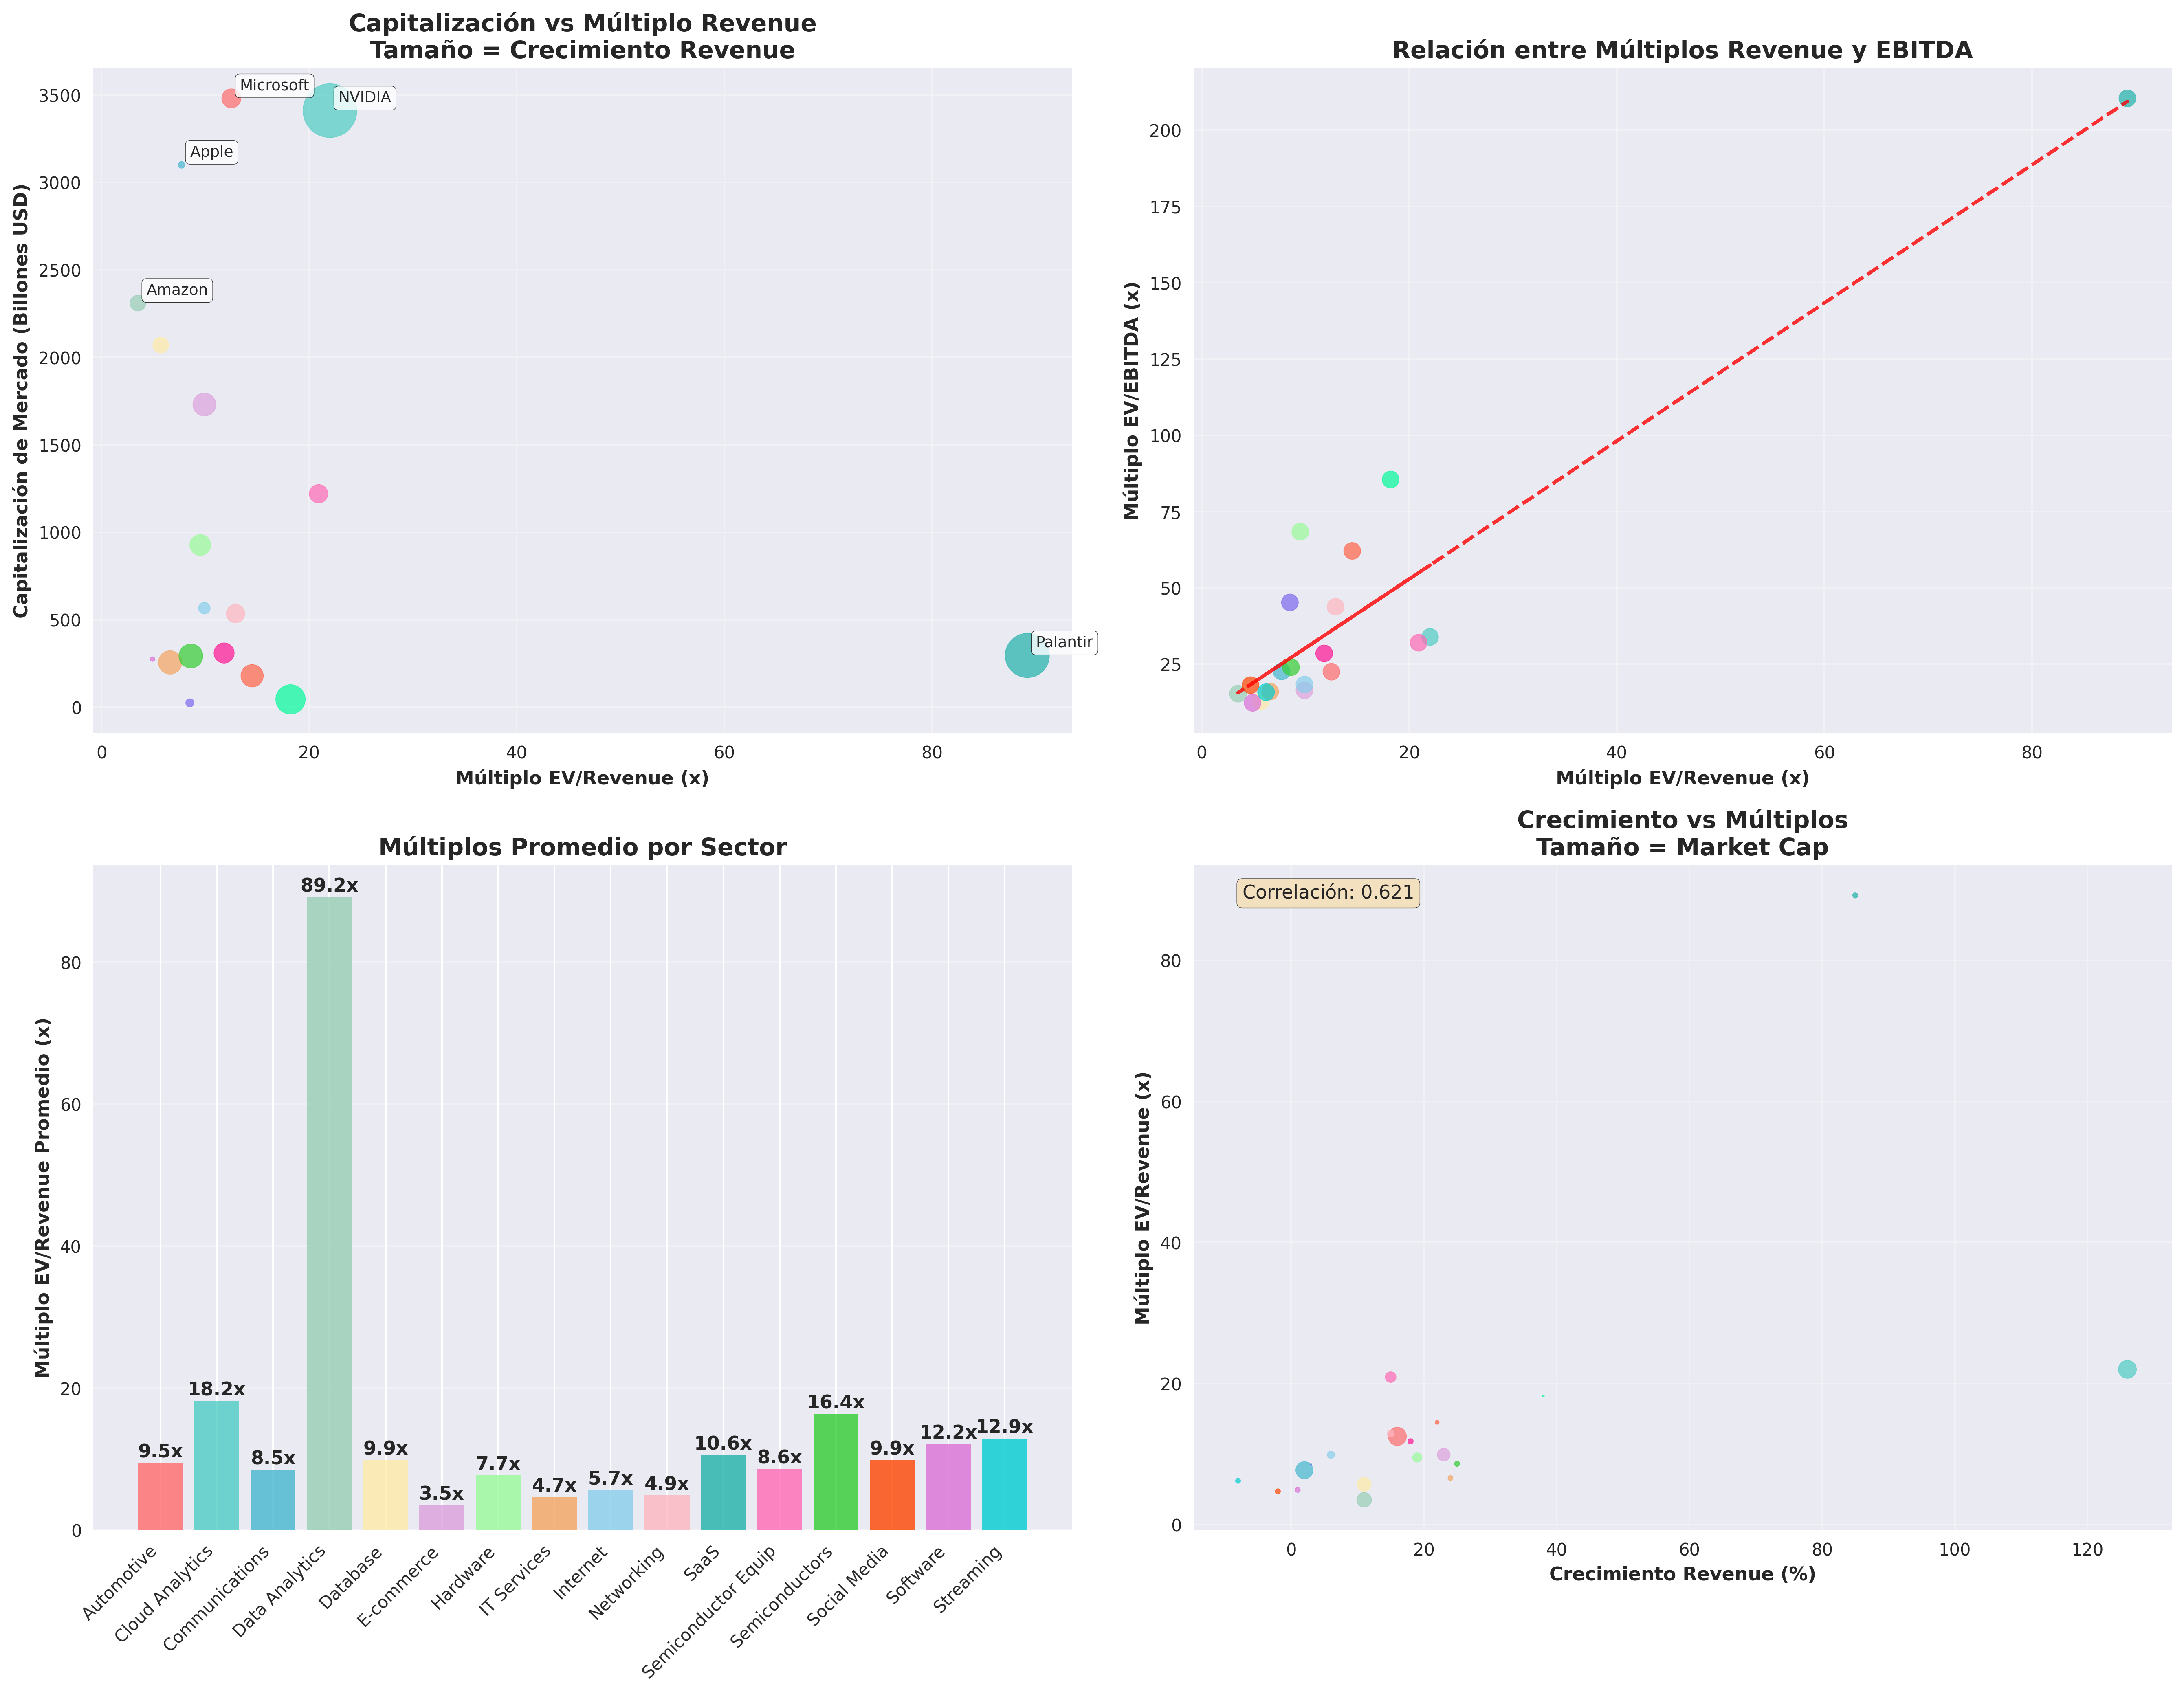
\includegraphics[width=0.9\textwidth]{figuras/analisis_empresas_lideres}
    \caption{Análisis comparativo de empresas tecnológicas líderes: capitalización de mercado, múltiplos de valoración y métricas de rentabilidad (2024)}
    \label{fig:comparacion_empresas}
\end{figure}

\begin{figure}[htbp]
    \centering
    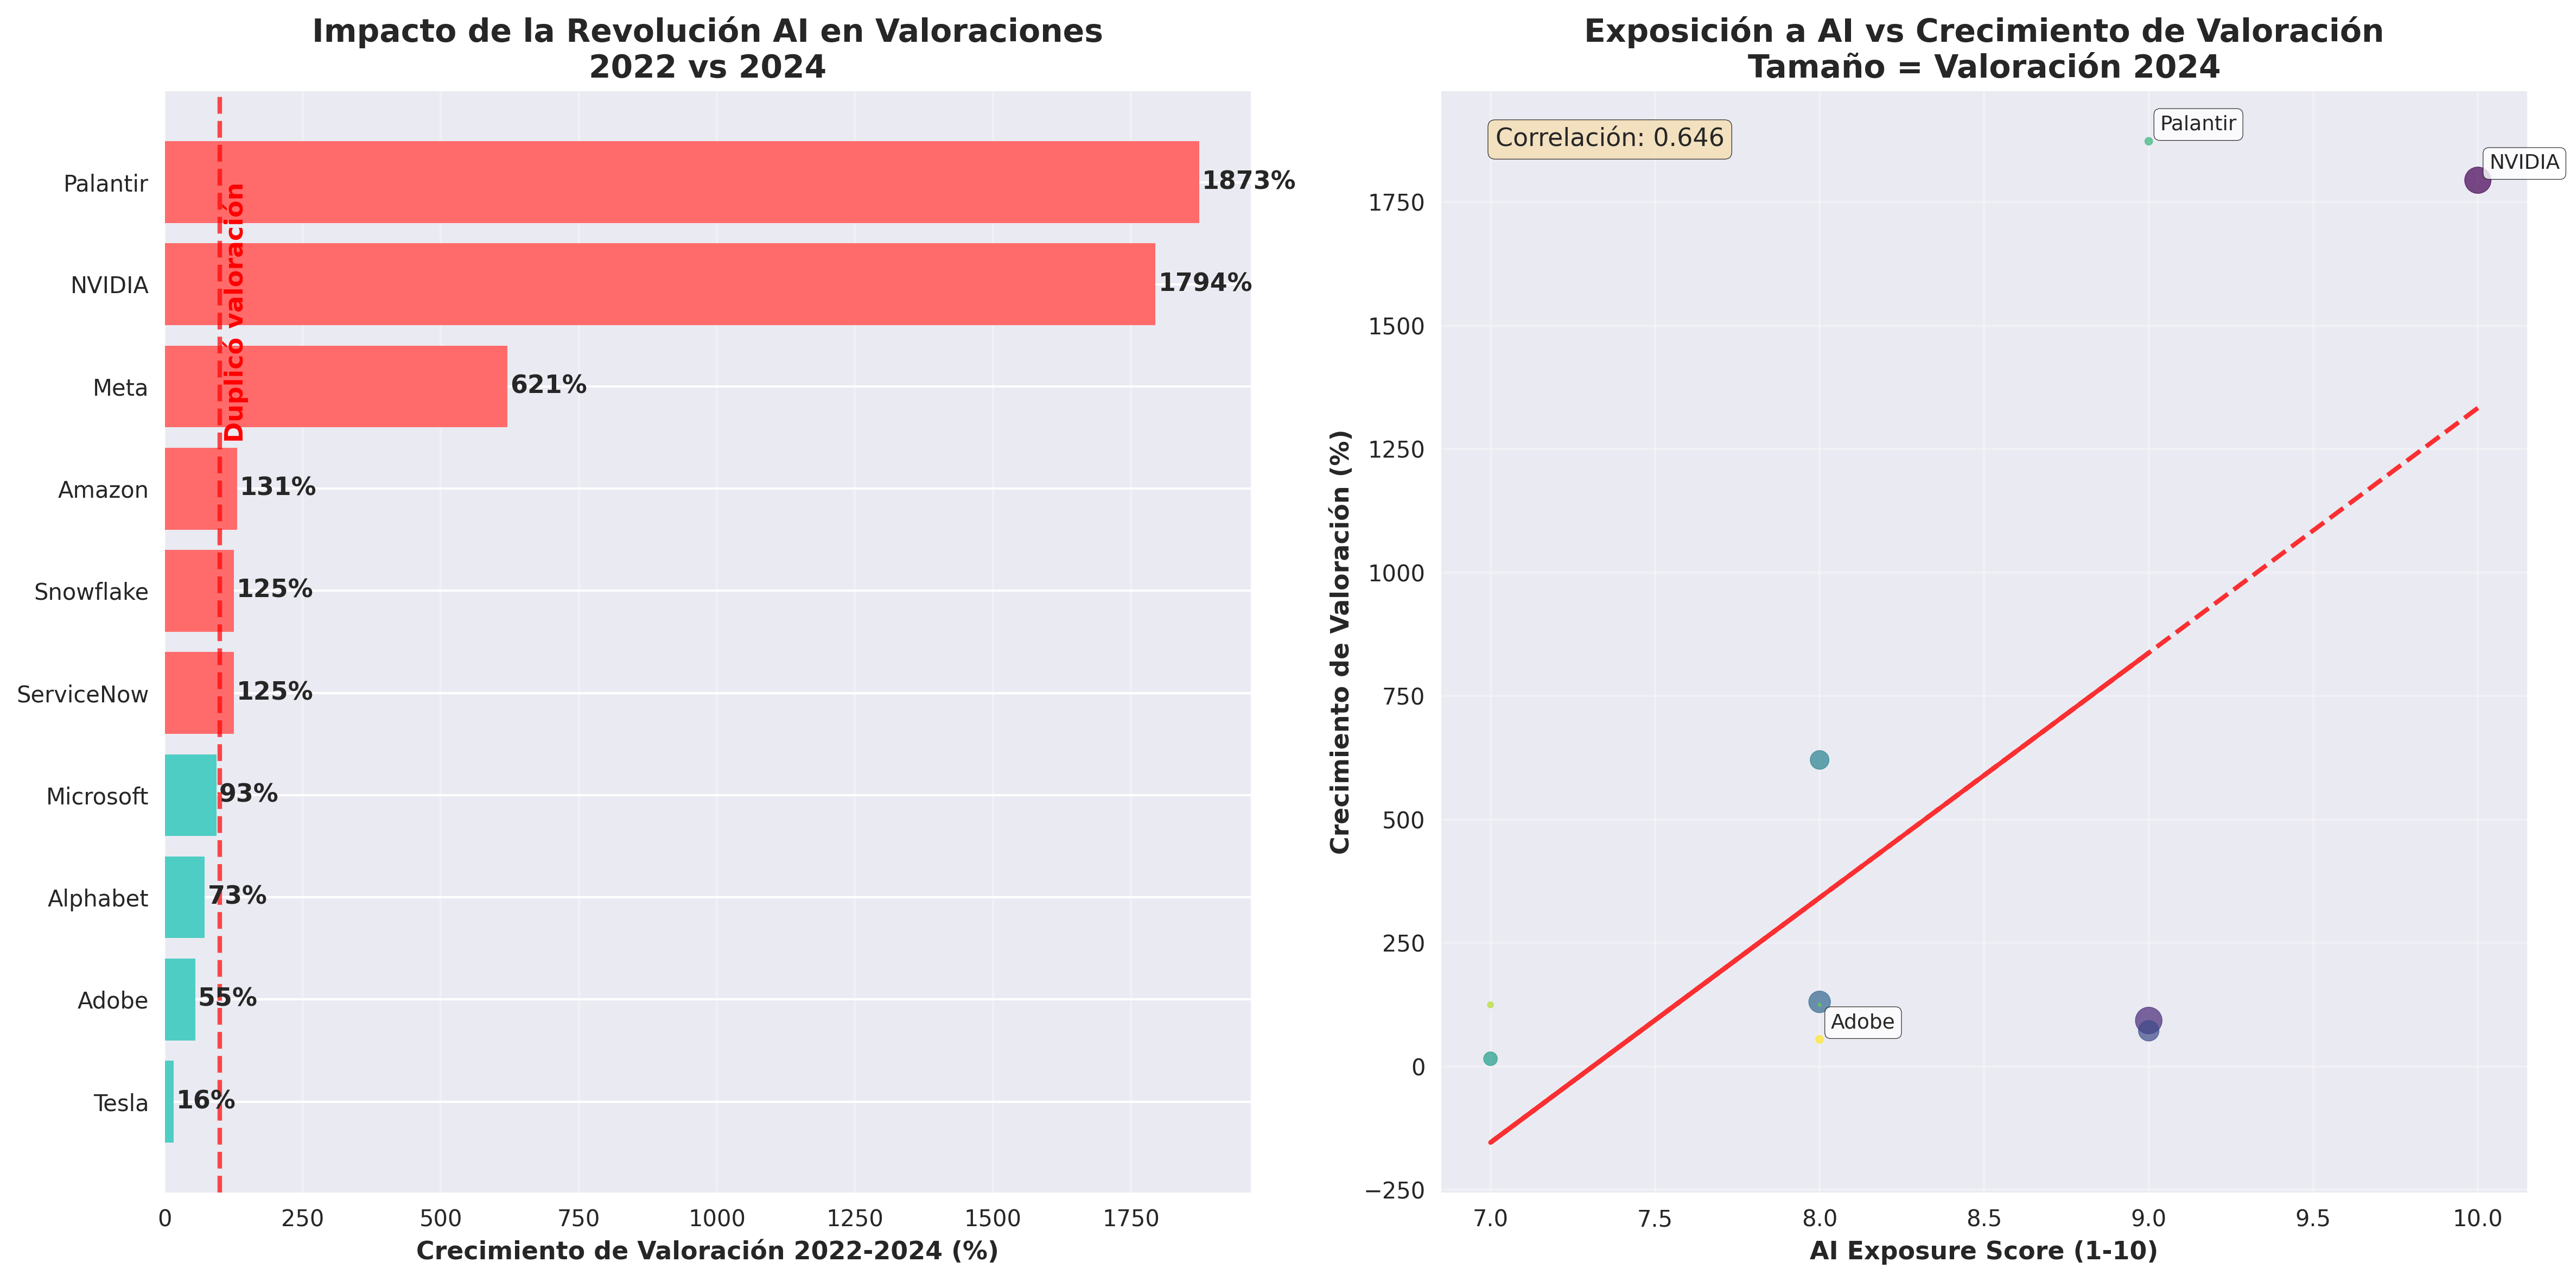
\includegraphics[width=0.9\textwidth]{figuras/impacto_ai_valoraciones}
    \caption{Impacto de la Inteligencia Artificial en valoraciones del sector tecnológico: crecimiento de capitalización y correlación con capacidades de IA (2022-2024)}
    \label{fig:impacto_ai}
\end{figure}

\subsection{Síntesis analítica de los casos}

Los casos estudiados ilustran lecciones fundamentales para la valoración de empresas tecnológicas que trascienden las particularidades individuales de cada empresa. Amazon demostró que el mercado puede respaldar estrategias de crecimiento a largo plazo cuando existe credibilidad demostrada en la capacidad de ejecución y una visión estratégica coherente respaldada por inversiones sustanciales en activos intangibles. Tesla ejemplificó cómo las narrativas de disrupción tecnológica pueden generar valoraciones que exceden considerablemente los fundamentos financieros actuales, reflejando expectativas especulativas sobre la materialización de mercados futuros y la monetización de opciones de crecimiento.

Google ilustró la importancia crítica de los activos intangibles superiores ---algoritmos, datos, efectos de red--- que pueden generar posiciones competitivas virtualmente dominantes y márgenes operativos excepcionales sostenibles a largo plazo. WeWork, por el contrario, subrayó que el mercado eventualmente exige coherencia entre la narrativa corporativa y la realidad operativa, y que las valoraciones basadas principalmente en expectativas sin fundamento empírico pueden colapsar dramáticamente cuando se exponen al escrutinio de inversionistas institucionales sofisticados.

El análisis contemporáneo de empresas en la era de la IA confirma que la diferenciación tecnológica real ---como la demostrada por NVIDIA en semiconductores especializados--- puede sostener múltiplos excepcionales cuando se combina con ejecución operativa sólida y barreras de entrada defendibles. Paralelamente, empresas como Palantir evidencian que el mercado continúa dispuesto a asignar valoraciones elevadas basadas en potencial futuro, aunque con niveles de riesgo proporcionalmente superiores reflejados en costos de capital más altos.

En síntesis, los casos analizados revelan que las empresas tecnológicas exitosas terminan validando sus valoraciones inicialmente elevadas a través de la materialización de crecimiento rentable sostenible y la demostración de ventajas competitivas duraderas, mientras que aquellas incapaces de demostrar viabilidad económica fundamental experimentan correcciones severas en sus valuaciones de mercado que pueden llegar hasta el colapso total del valor. 